\documentclass[a4paper,12pt,article]{memoir}
\usepackage{amsmath}
\usepackage{amssymb}
\usepackage{mathspec}
\usepackage{xltxtra}
\usepackage{polyglossia}
\usepackage{MnSymbol}
\usepackage{siunitx,cancel,graphicx}
\usepackage{enumitem}
\usepackage{hyperref,graphicx}
\usepackage{icomma}
\usepackage{float}
\usepackage{mleftright}

\usepackage{listings}
\usepackage{color}



% This is the color used for MATLAB comments below
\definecolor{MyDarkGreen}{rgb}{0.0,0.4,0.0}
\definecolor{Blue}{rgb}{0.0,0.0,1.0}
\definecolor{Purple}{rgb}{1.0,0.0,1.0}

\lstset{language=c,
                basicstyle=\ttfamily,
                keywordstyle=\color{blue}\ttfamily,
                stringstyle=\color{red}\ttfamily,
                commentstyle=\color{green}\ttfamily,
                morecomment=[l][\color{magenta}]{\#},
                breaklines=true,
                frame=single
}

\setdefaultlanguage{english}

\defaultfontfeatures{Scale=MatchLowercase,Mapping=tex-text}
%\setmainfont[Numbers=Lowercase]{Minion Pro}
%\setsansfont[Numbers=Lowercase]{Myriad Pro}
%\setmonofont{Menlo}
%\setmathsfont(Digits,Latin,Greek)[Numbers={Lining,Proportional}]{Minion Pro}

\sisetup{%
  output-decimal-marker = {,},
  per-mode = symbol,
  %round-mode = places,
  %round-precision = 5
}



\setlrmarginsandblock{2.5cm}{2.5cm}{*}
\setulmarginsandblock{1.5cm}{2cm}{*}
\checkandfixthelayout

\setlength{\parindent}{2em}
\setlength{\parskip}{0pt}

\newcommand{\f}{\fancybreak}

\DeclareSIUnit \electronvolt {\ensuremath{eV}}

\newcommand{\mvec}[2]{
\ensuremath{\left(
\begin{array}{c}
#1\\
#2\\
\end{array}
\right)}
}

\newcommand{\Span}{\ensuremath{\mathrm{Span}}}
\newcommand{\Mat}{\ensuremath{\mathrm{Mat}}}
\newcommand{\C}{\ensuremath{\mathbb{C}}}
\newcommand{\Q}{\ensuremath{\mathbb{Q}}}
\newcommand{\Gr}{Gröbner\ }
\newcommand{\R}{\ensuremath{\mathbb{R}}}
\newcommand{\N}{\ensuremath{\mathbb{N}}}
\newcommand{\Rno}{\ensuremath{\mathbb{R}\backslash\{0\}}}
\newcommand{\Z}{\ensuremath{\mathbb{Z}}}
\newcommand{\ol}[1]{\ensuremath{\overline{#1} } }
\newcommand{\F}[1]{\ensuremath{\mathbb{F}_{#1} } }

\title{Latex Exercise}
\author{Nikolaj Roager Christensen: student ID 201805275}
\date{2022 CE} %

\begin{document}

\maketitle

\chapter*{An approximation for the exponential function}
This should solve part A and B, as C is optional and don't give any points I honestly don't care

Table \ref{tab:code} shows a possible numerical implementation of the Exponential function in the c\#


\begin{table}
\begin{lstlisting}
static double ex(double x)
{
    if(x<0)          //Adjust the approximation to be positive
        return 1/ex(-x);
    if(x>1.0/8)
        return Pow(ex(x/2),2);//and "small", note I am using 2 and not 2.0
    //Now use the approximation
    return 1+x*(1+x/2*(1+x/3*(1+x/4*(1+x/5*(1+x/6*(1+x/7*(1+x/8*(1+x/9*(1+x/10)))))))));
}
\end{lstlisting}
\caption{A simple approximation of the exponential function, using only multiplication and division (the mono c\# compiler do interpret \lstinline{System.Math.Pow(double,int)} as a list of mulitiplications). }
\label{tab:code}
\end{table}


This function does two things, firstly it re-adjust the input x to be between 0 and $1/8$, and secondly it calculates a reasonable approximation.

Setting aside the re-adjustment for now, we know that the taylor-expansion of $\exp(x)$ around $x=0$ is

\begin{equation}
\exp(x) = \sum_{n=0}^\infty \frac{x^n}{n!}.
\end{equation}

For $x\approx 0$ it is a reasonable approximation to only use the first few terms, in this case we use the first 11 terms up until $n=10$.

\begin{align}
\exp(x) &\approx \sum_{n=0}^{10} \frac{x^n}{n!}.
\end{align}

The error made here is on the order $O(x^{11})$, if only the user asked us for small $x$ this would be very reasonable. In practice we want to reduce the number of multiplications used, and we can do that since:


\begin{align}
\exp(x) &\approx \sum_{n=0}^{10} \frac{x^n}{n!},\\
 &\approx 1+\sum_{n=1}^{10} \frac{x^n}{n!},\\
 &\approx 1+\frac{x}{1}\sum_{n=0}^{9} \frac{x^n}{(n+1)!}.
\end{align}

We can repeat the same trick 9 times on the sum, the result is:

\begin{align}
\exp(x) &\approx  1+\frac{x}{1}\left(1+\frac{x}{2}\left(1+\frac{x}{3}\left(\ldots\left(1+\frac{x}{9}\right)\right)\right)\right).
\end{align}

Now we just have 10 additions 9 divisions and 9 multiplications, which is considerably better, and this is the approximation used in Table \ref{tab:code}.

In Figure \ref{fig:exp} (a), this approximation is illustrated alongside the exponential function (b). Of course, we still need to have $x$ relatively close to 0, as is evident on the figure the approximation diverges for $x$ not close to $0$. This can be fixed by using the relation $\exp(x/2)^2=\exp(x)$ which is applied (recursively) whenever $x>1/8$ to get within this range, if $x<0$ we do know that $\exp(x)=1/\exp(-x)$, where $-x$ is positive; making sure the argument is positive is necessary in order for the other check ($x>1/8$) to be applied. So the two first if-statements simply make sure that we are within the range $[0,0.125]$. This is illustrated in Figure \ref{fig:exp} (c). This ensures that the approximation always is applied when $x$ is within where it should remain valid.

\begin{figure}
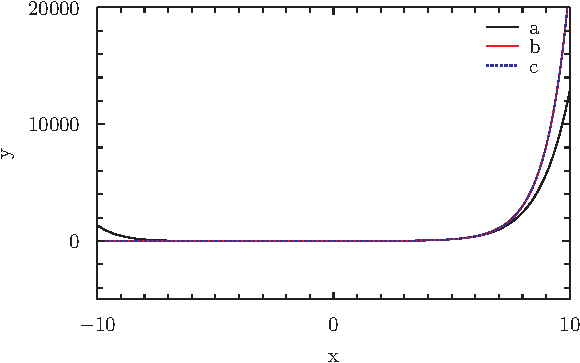
\includegraphics[width = 0.5\linewidth]{exp.pdf}
\caption{(a) the approximation without correcting the range, (b) the true exponential function and, (c) the approximation correcting $x$ to be within a reasonable range.}
\label{fig:exp}
\end{figure}

\end{document}

